\chapter{Arquitetura da Solução}
\label{chapter:Arquitetura}
\noindent

\section{Fluxo de atividades}

\begin{figure}[!ht]
	\centering
	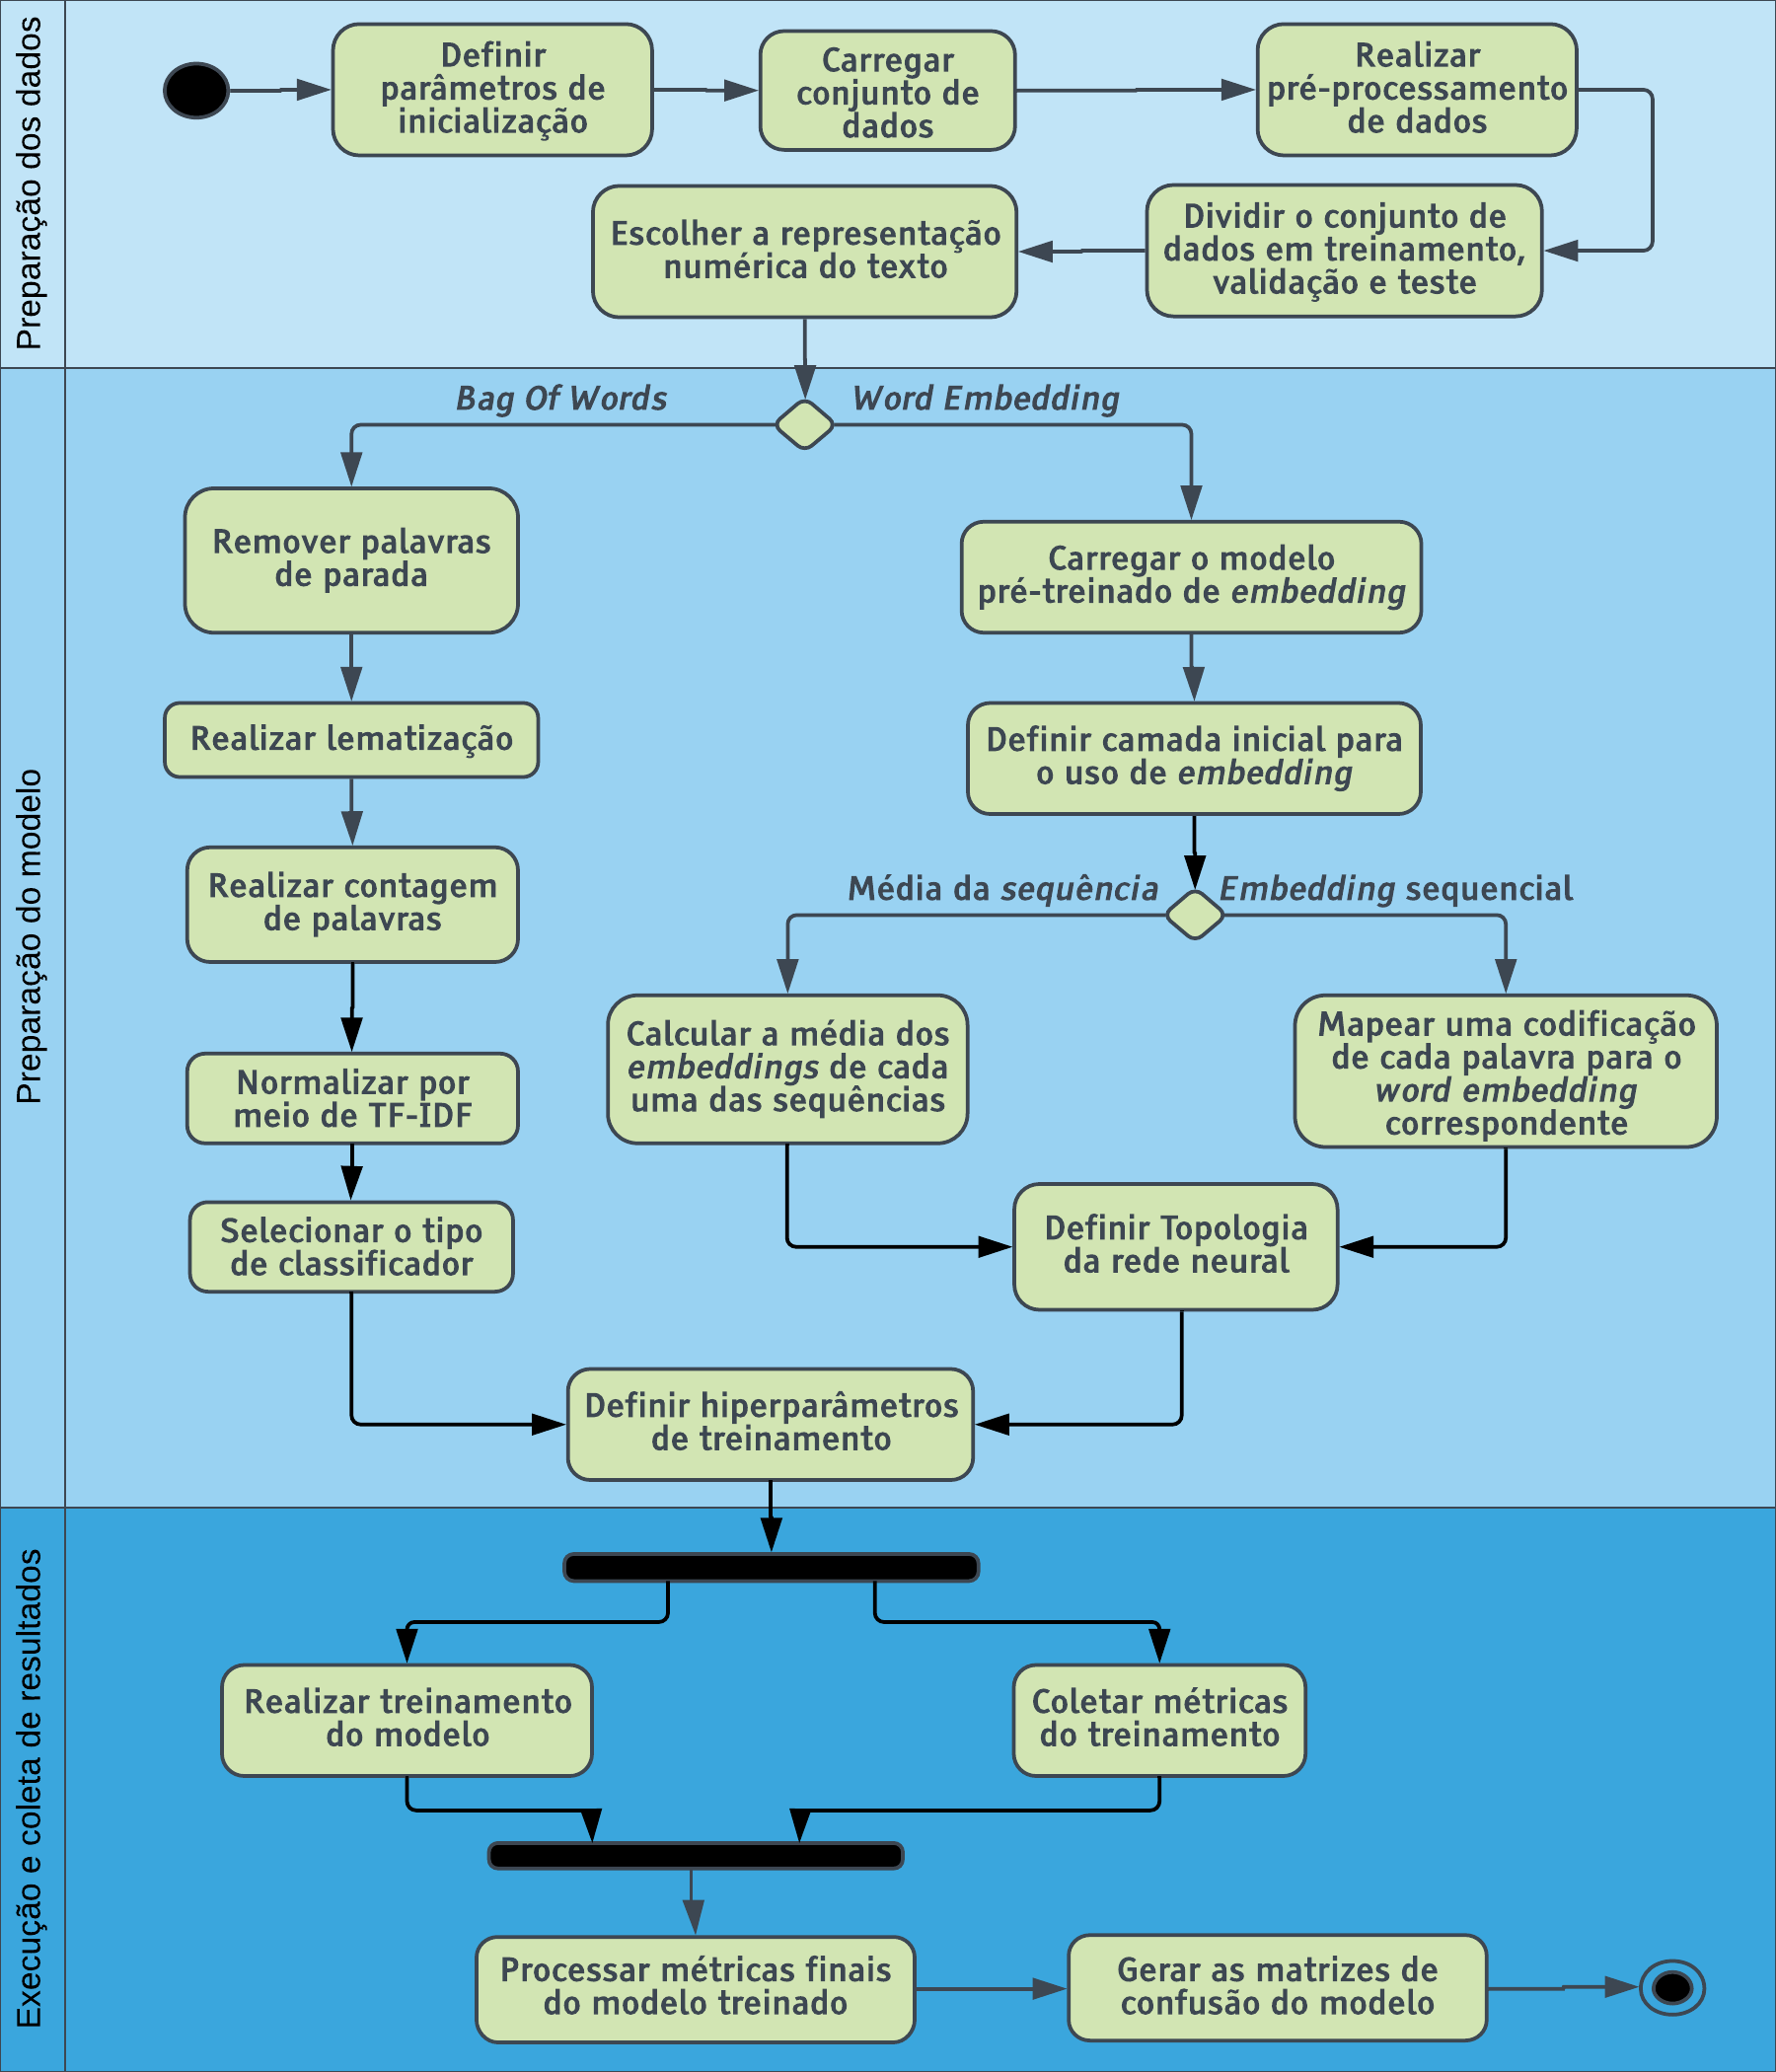
\includegraphics[width=1.1\textwidth]{figures/ActivityDiagram.png}
	\caption{Diagrama de atividades}
	\label{fig:ActivityDiagram}
\end{figure}

Antes de se discutir detalhes técnicos da implementação, é interessante definir um fluxo de operações que serão realizadas pelo sistema. Isso permite uma melhor contextualização geral das funcionalidades a serem implementadas não só por quem participará da sua implementação, mas também por quem será seu usuário.

Uma primeira observação sobre esse fluxo de atividades é que ele é posterior à fase de obtenção de dados descrita no capítulo \ref{chapter:ObtencaoBases}. A razão disso é porque a arquitetura descrita no presente capítulo independe da fonte de dados utilizada, buscando uma fácil portabilidade para outros contextos de classificação de texto.

Todas as etapas a serem implementadas pelo sistema são descritas no diagrama de atividades da figura \ref{fig:ActivityDiagram}. Esse diagrama pode ser resumido em três estágios principais: uma fase inicial de preparação dos dados; uma segunda fase que define o modelo do classificador e executa as etapas que precedem o treinamento;  e uma fase final em que é realizado o treinamento do modelo especificado no estágio anterior assim como são coletadas métricas sobre sua performance.

\section{Modelagem da Implementação}

\begin{figure}[!ht]
	\centering
	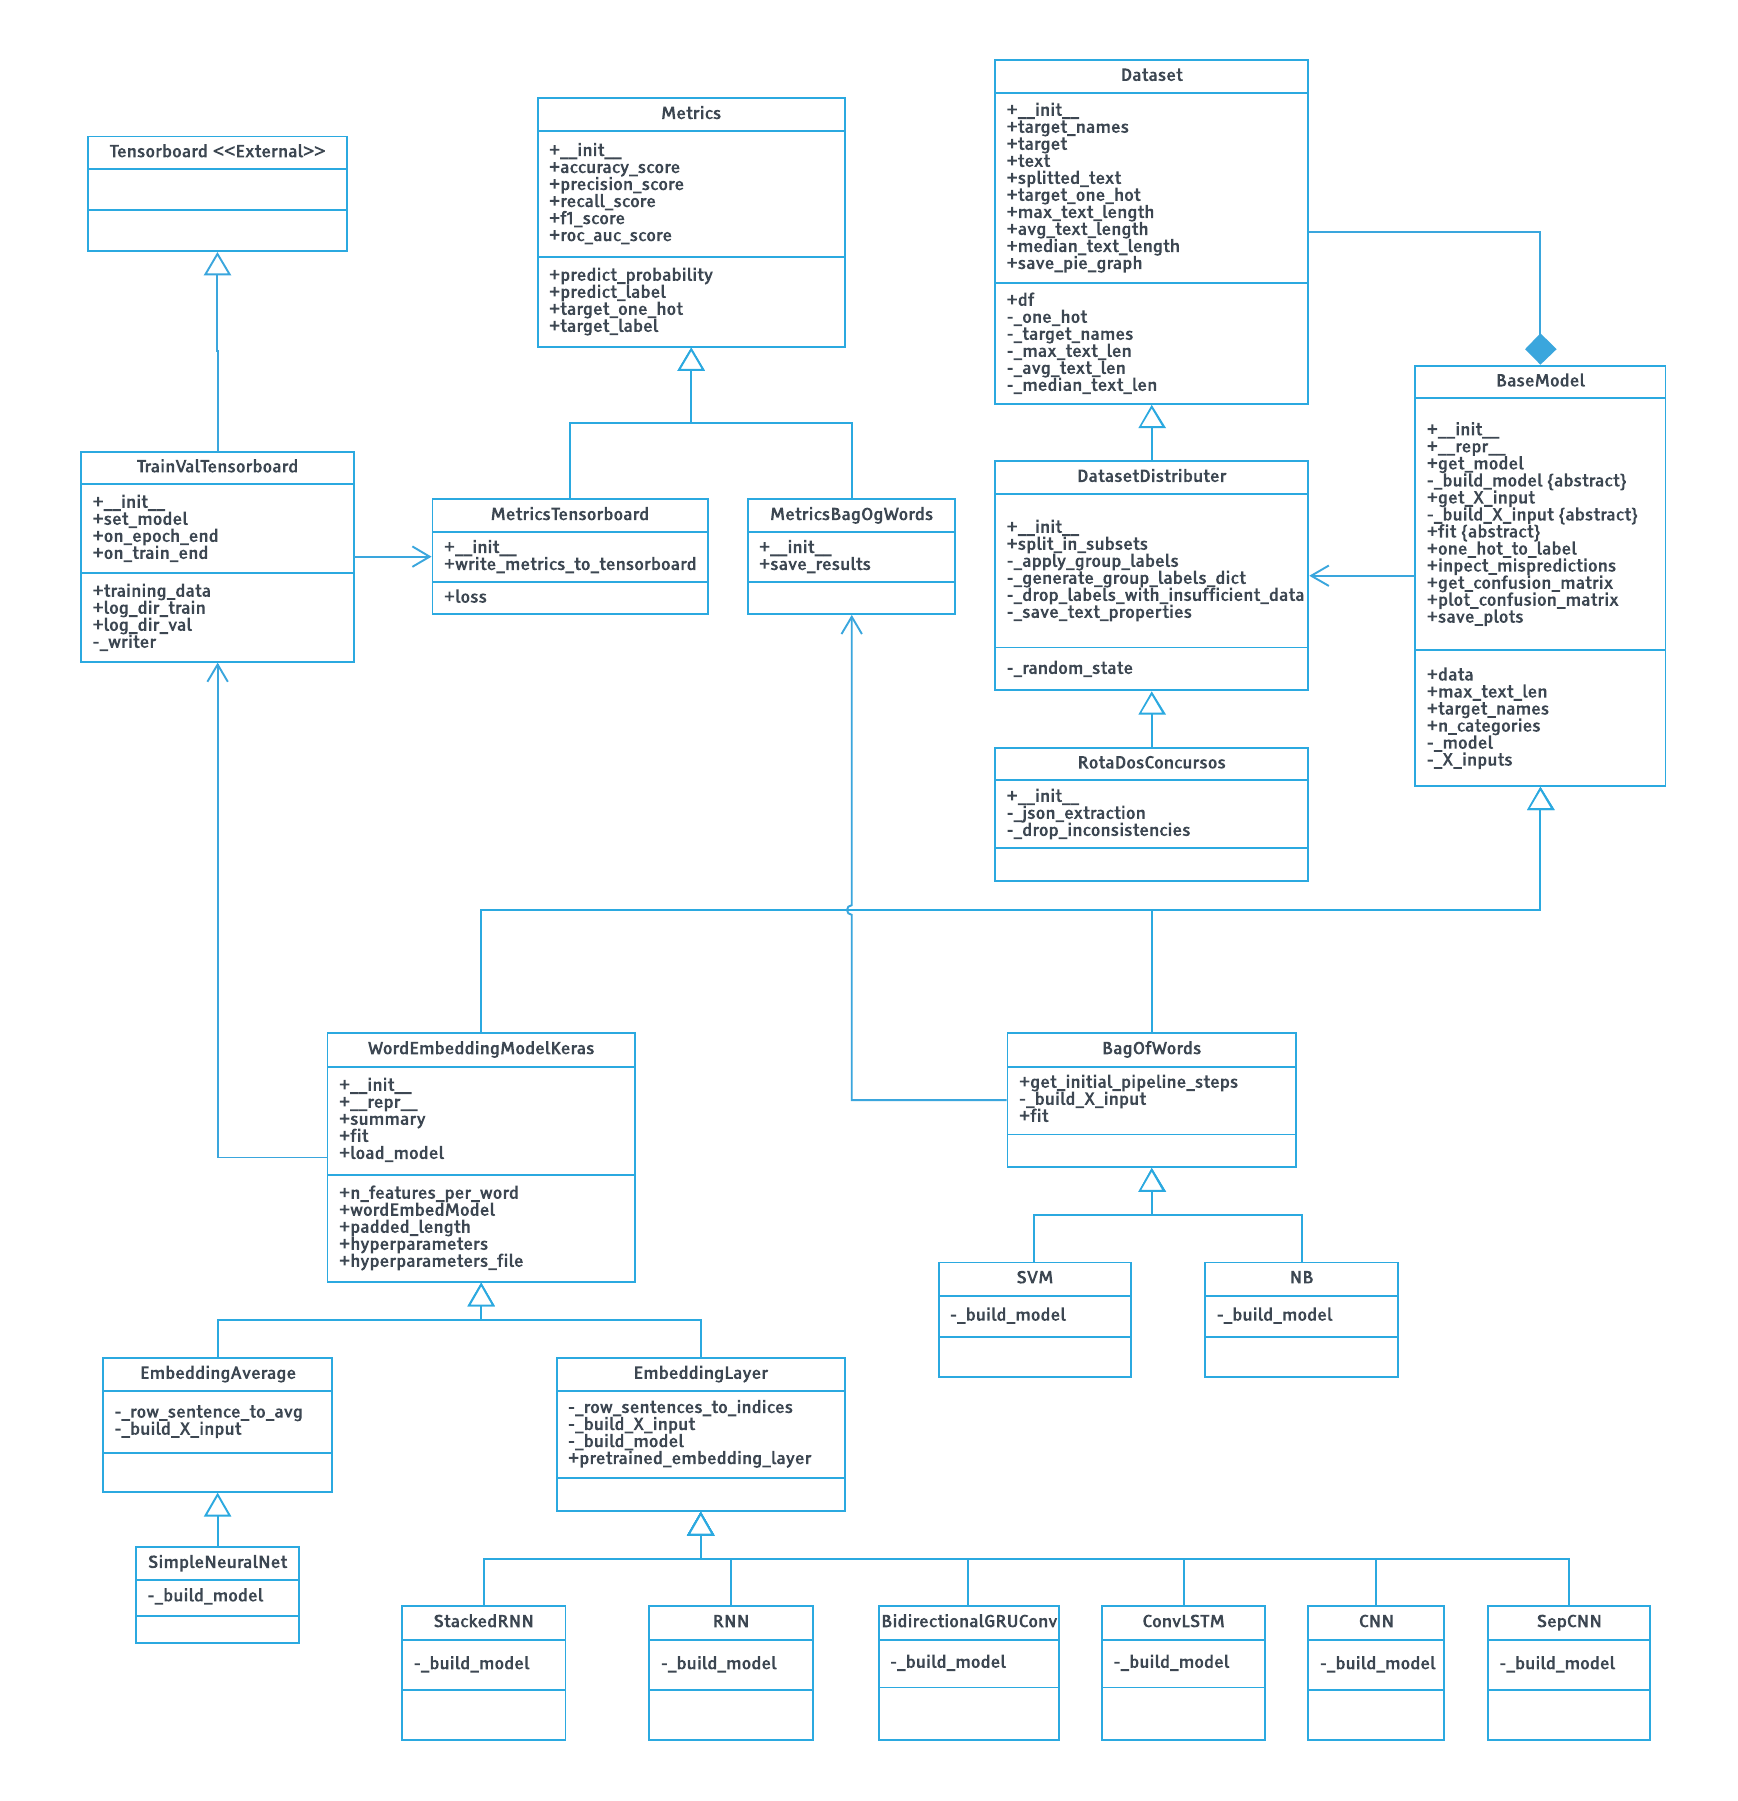
\includegraphics[width=1.15\textwidth]{figures/ClassDiagram.png}
	\caption{Diagrama de classes}
	\label{fig:ClassDiagram}
\end{figure}

Nas implementações dos classificadores, existem várias etapas em comum conforme já ilustrado pela figura \ref{fig:ActivityDiagram}. Em virtude disso, buscou-se realizar uma implementação que satisfizesse requisitos de manutenibilidade e reusabilidade. Dessa forma, foi elaborada uma solução focada em uma hierarquia de classes que maximizasse o reúso de implementações entre os modelos conforme ilustra o diagrama de classes na figura \ref{fig:ClassDiagram}. 

Essa arquitetura modulariza as etapas do sistema. Um dos aspectos que se buscou dar destaque nessa modularização foi o processamento da fonte de dados, isso é feito de maneira isolada em uma classe específica que pode ser facilmente substituída por outra que implemente o carregamento de dados de outra fonte. No diagrama de classes da figura \ref{fig:ClassDiagram}, essa classe corresponderia a uma que substituiria a classe \hl{RotaDosConcursos}, mantendo a mesma interface. Para tanto, essa nova classe também deve herdar de \hl{DatasetDistributer}. Depois disso, bastaria passar um objeto dessa nova classe ao instanciar um objeto correspondente a um classificador genérico que é implementado pela classe hl{BaseModel}. Isso ocorre porque a classe \hl{BaseModel} trata o objeto correspondente aos dados no seu construtor apenas no nível da classe \hl{DatasetDistributer}.

Quanto a implementação dos modelos, também trabalhou-se buscando uma modularidade para dar suporte a adição de novos classificadores. Antes no entanto, discutiremos qual o significado dos níveis da hierarquia de classes que implementa essa solução.

Primeiramente, parte-se da classe abstrata \hl{BaseModel} que, conforme já mencionado, implementa operações comuns a todos os modelos como métodos relacionados à exibição de resultados e à admissão de dados. Essa classe é então especializada de acordo com as duas estruturas de dados para a representação de texto em concordância com as definições do capítulo \ref{cap:methods} e também ilustradas no primeiro \textit{fork} da figura \ref{fig:ActivityDiagram}. Assim, o segundo nível dessa hierarquia é composto pelas classes \hl{BagOfWords} e \hl{WordEmbeddingModelKeras}.

Em seguida, no caso de modelos que partem da representação \textit{Bag of Words}, especializa-se de acordo com o algoritmo classificador a ser utilizado, sendo este o último nível. Já para modelos baseados em \textit{Word Embedding}, esse é o penúltimo nível e corresponde ao segundo \textit{fork} (de cima para baixo) na figura \ref{fig:ActivityDiagram}. Vale ressaltar que apesar de somente duas abordagens para o uso da representação por \textit{Word Embedding} serem exploradas, a adição de mais uma versão seria simples graças ao isolamento dessa etapa em uma única classe que se integra ao restante da arquitetura por meio de herança. A última especialização do ramo referente a \textit{Word Embedding} define a topologia da rede neural implementada. Para os dois ramos, novos classificadores podem ser facilmente adicionados ao último nível devido a flexibilização dessa arquitetura modular. Contudo, há algumas ressalvas, a primeira delas é que esse projeto trabalha apenas com redes neurais para a representação \textit{Word Embedding}, assim o último nível é, conforme já foi dito, responsável apenas pela definição topológica. Além disso, a implementação foi todo feita em \textit{Python} e essa topologia deve ser feita utilizando a API \textit{Keras} do pacote \textit{Tensorflow} e o classificador utilizado na representação \textit{Bag of Words} deve seguir a interface do pacote \textit{Scikit-learn}.

Por fim há ainda um conjunto de classes que trabalha a definição das métricas que são coletadas. As mesmas métricas são coletadas independentemente da representação numérica utilizada para o texto. Contudo, algumas especializações são feitas porque os recursos de visualização do \textit{Tensorboard}, com compatibilidade exclusiva para o pacote \textit{Tensorflow}, foram explorados somente para os modelos que partem da representação \textit{Word Embedding}.

\section{Aspectos Práticos da Implementação}

Um aspecto da implementação que foi de grande importância na viabilização da execução dos treinamentos foi a facilidade de se utilizar vários núcleos de processamento ao utilizar a biblioteca como \textit{scikit-learn}. Isso permitiu a paralelização utilizando vários núcleos de um servidor robusto do serviço AWS da \textit{Amazon} conforme ilustra a figura \ref{fig:paralelization_AWS}. Além disso, o pacote \textit{Tensorflow} abstrai o uso de GPUs em um alto nível, o que também foi explorado ao utilizar os serviços da AWS.

\begin{figure}[!ht]
	\centering
	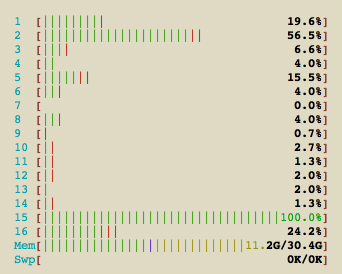
\includegraphics[width=0.6\textwidth]{figures/htop.png}
	\caption{Uso das CPUs no servidor durante um dos treinamentos}
	\label{fig:paralelization_AWS}
\end{figure}

Vale destacar que o uso dos serviços AWS foi completamente automatizado. Isso significa que foi implementado um \textit{script} que realiza as seguintes operações: definição de toda a configuração da máquina virtual; criação de uma nova instancia dessa máquina; realização do \textit{download} do conjunto de dados preparado conforme descrito no capítulo \ref{chapter:ObtencaoBases} que foi disponibilizado publicamente em um servidor de armazenamento também da \textit{Amazon}; realização do download do modelo de \textit{Word Embedding} disponibilizado como parte do trabalho do artigo \cite{DBLP:journals/corr/abs-1708-06025}; download do código do modelo implementado como parte do presente trabalho; execução do treinamento de um modelo selecionado; exportação das métricas para o armazenamento em nuvem \textit{S3} da \textit{Amazon}; terminação da instância da VM criada.

Por fim, visando a rastreabilidade das alterações do código durante o desenvolvimento e uma colaboração em equipe, todo o código foi versionado. O repositório pode ser acessado em: github.com/brunovcosta/pfc .
